
% !TEX program = pdflatex
% !TEX enableSynctex = true
% !BIB program = bibtex


\documentclass[12pt]{article}

\usepackage{setspace}
\usepackage{amsmath}
\usepackage{amsfonts}
\usepackage{graphicx}
\usepackage{float}
\addtolength{\oddsidemargin}{-.7in}
\addtolength{\evensidemargin}{-.7in}
\addtolength{\textwidth}{1.4in}
\usepackage{enumerate}
\onehalfspacing
\usepackage{geometry} % Required for customizing page layout

\usepackage{caption}
\usepackage{booktabs}

\usepackage{hyperref}
\hypersetup{
	pdfstartview = FitH,
	pdfauthor = {...},
	pdftitle = {...},
	pdfkeywords = {...; ...; ...; ...},
	colorlinks = true,
	linkcolor = blue,
	urlcolor = blue,
	citecolor = blue,
	linktocpage=true
}


\begin{document}
\section*{Partial equilibrium model - firms' problem}
\subsection*{Ver 1 - PE model - Fixed q-s - 3 state variables}
Productivity process: two-state markov chain \vspace{3mm} \\
Labour policy: 
\begin{equation}
    n(k,\varepsilon_i) = \left( \dfrac{ \nu \varepsilon_i k^\alpha}{w} \right)^{\frac{1}{1-\nu}}
\end{equation}
Corresponding output: 
\begin{equation}
    y(k,\varepsilon_i) = \varepsilon_i k^{\alpha} \left( \dfrac{\nu \varepsilon_i k^\alpha}{w} \right)^{\frac{\nu}{1-\nu}}
\end{equation}
Corresponding profits: 
\begin{equation}
    \pi(k,\varepsilon_i) = (1-\nu) y(k,\varepsilon_i) - c
\end{equation}
External finance premium - just a parameter \vspace{2mm} \\
Value function:
\begin{equation}
     V(k,b, \varepsilon_i) = \max_{k',b'}  \left( \pi(k,\varepsilon_j)+(1-\delta)k - k' +  q^s b' -b  +
            \beta (1-P_\chi) \sum_{j=1}^{N_\varepsilon} g_{ij}  V(x',\varepsilon_j') \right)
\end{equation}
\noindent Here, the firm can directly choose $k'$ and $b'$, which makes coding the transition matrix easier, since you do not have to interpolate the Q-es. In the end you just have some very sparse matrices, since the model is almost deterministic. \vspace{3mm} \\
The shortcoming is you have 3 state variables and 2 action variables, which means that it is very hard to move past a grid size of 30. 

\newpage
\setcounter{equation}{0}


\subsection*{Ver 2 - Fixed Qs - cash on hand - two-state productivity}
Productivity process: two-state markov chain \vspace{3mm} \\
Labour policy: 
\begin{equation}
    n(k,\varepsilon_i) = \left( \dfrac{ \nu \varepsilon_i k^\alpha}{w} \right)^{\frac{1}{1-\nu}}
\end{equation}
Corresponding output: 
\begin{equation}
    y(k,\varepsilon_i) = \varepsilon_i k^{\alpha} \left( \dfrac{\nu \varepsilon_i k^\alpha}{w} \right)^{\frac{\nu}{1-\nu}}
\end{equation}
Corresponding profits: 
\begin{equation}
    \pi(k,\varepsilon_i) = (1-\nu) y(k,\varepsilon_i) - c
\end{equation}
Future cash on hand: 
\begin{equation}
   x' = \pi(k',\varepsilon_j')+(1-\delta)k'-b'
\end{equation}
External finance premium 
\begin{equation}
    q^s = 0.94
\end{equation}
Need an equity finance option. Otherwise there certain states are not associated to any feasible action. Here, I assume. This means that firms will sometimes have negative cash on hand. 
\begin{equation}
    d < 0 \implies d = 1.6d
\end{equation}
Value function:
\begin{equation}
     V(x,\varepsilon_i) = \max_{k',b'}  \left(x - k' +  q^s b' + 
            \beta  (1-P_\chi)  \sum_{j=1}^{N_\varepsilon} g_{ij} V(x',\varepsilon_j') \right)
\end{equation}
Adding cash on hand reduces the grid to 2 state and 2 action variables. This implies that you can do a much larger grid. However, you have to interpolate resulting x that follows from choices k' and b' to the grid, since x-here is the result. This could be a problem. Generally, results are well behaved in this case, although they are very mechanical. 


\begin{figure}[H]  % [h] indicates placing the image here
    \centering
    \caption{Ver2 - prod: 5, 8} \label{chart:CFLcdf}
    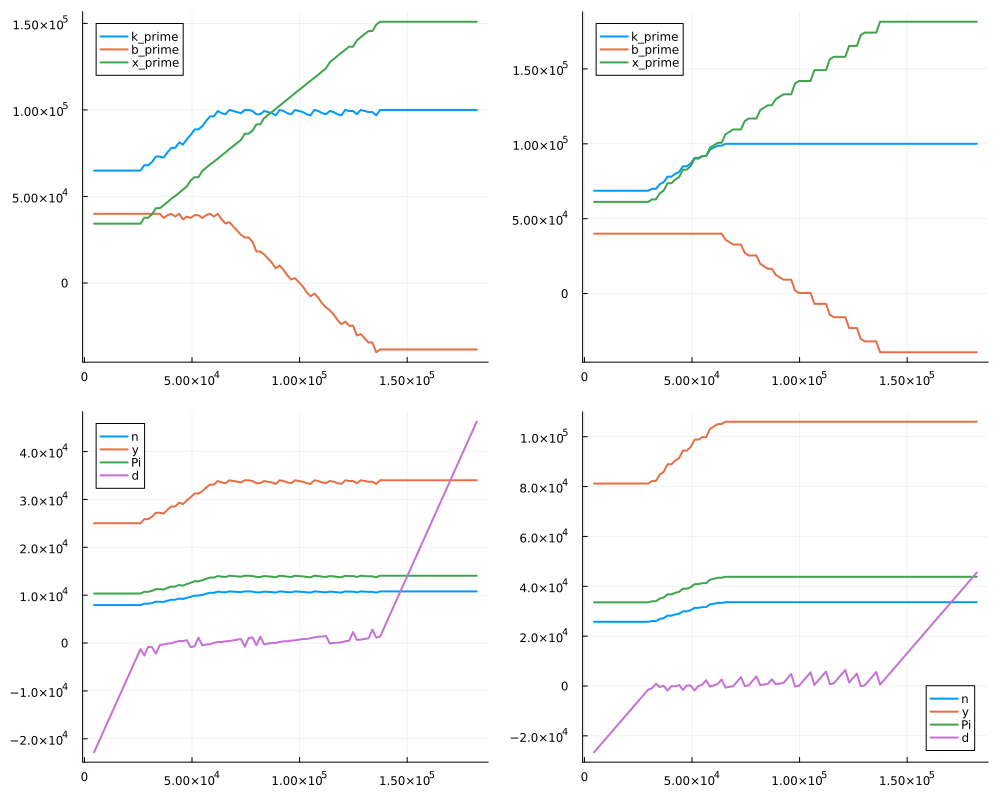
\includegraphics[width=1\textwidth]{ver2.png}
\end{figure}


\newpage
\setcounter{equation}{0}

\subsection*{Ver 3 - ABL Qs - cash on hand - AR(1) productivity}
Productivity process: AR(1) process with multiple states. Below, I plot the worst the median and the best productivity state. \vspace{3mm} \\
Labour policy: 
\begin{equation}
    n(k,\varepsilon_i) = \left( \dfrac{ \nu \varepsilon_i k^\alpha}{w} \right)^{\frac{1}{1-\nu}}
\end{equation}
Corresponding output: 
\begin{equation}
    y(k,\varepsilon_i) = \varepsilon_i k^{\alpha} \left( \dfrac{\nu \varepsilon_i k^\alpha}{w} \right)^{\frac{\nu}{1-\nu}}
\end{equation}
Corresponding profits: 
\begin{equation}
    \pi(k,\varepsilon_i) = (1-\nu) y(k,\varepsilon_i) - c
\end{equation}
Future cash on hand: 
\begin{equation}
   x' = \pi(k',\varepsilon_j')+(1-\delta)k'-b'
\end{equation}
External finance premium:
\begin{equation}
    q^{abl}(k',b')b' = \beta \left[ (1-P_\chi) b' + P_\chi \min\{b', \ \phi_k (1-\delta) k' \} \right]  
\end{equation}
Equity finance option:
\begin{equation}
    d < 0 \implies d = 1.6d
\end{equation}
Value function:
\begin{equation}
     V(x, \varepsilon_i) = \max_{k',b'}  \left( x - k' +  q(k',b',\varepsilon) b' +
            \beta (1-P_\chi) \sum_{j=1}^{N_\varepsilon} g_{ij}  V(x',\varepsilon_j') \right)
\end{equation}
Here the two innovations are that interest rates are endogenous and the productivity process is more realistic. Results makes sense, although they display this jigsaw pattern in certain regions and calibrations. \textbf{Weirdly, the model breaks down when grids are defined logarithmically.} Firms very quickly converge to their desired level of capital, even if they are cash-poor - that is because $q$ remains relatively large even for very indebted firms.

\begin{figure}[H]  % [h] indicates placing the image here
    \centering
    \caption{Ver3 - worst, median and best productivity states} \label{chart:CFLcdf}
    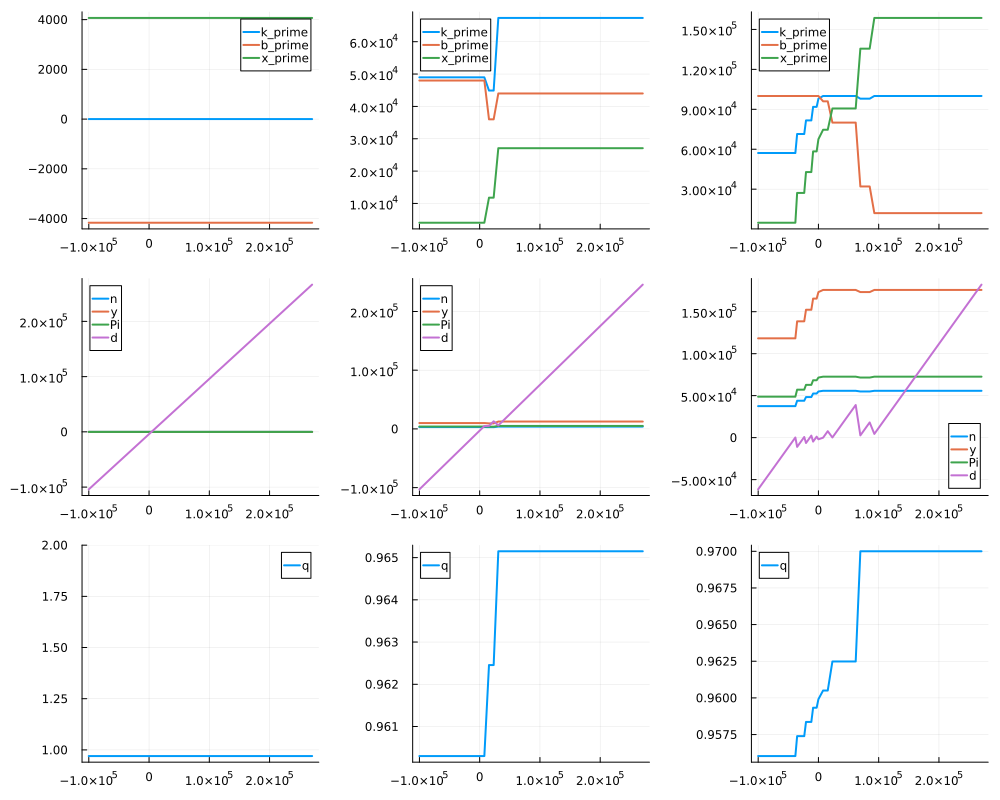
\includegraphics[width=1\textwidth]{ver3.png}
\end{figure}


\newpage

\section*{Summary of models up to Ver 3}

Measure of size problem: 
\begin{itemize}\setlength{\itemsep}{0pt}
    \item The problem with the cash on hand approach is that it does not have a good measure of current size. The current cash on hand might be misleading since large debt might cancel out large capital stocks.
    \item The best solution is to interpret everything in terms of next period's capital or production. This is ok but only if there is is a proper dispersion of capital stocks.
\end{itemize} 
On interest rates:
\begin{itemize}\setlength{\itemsep}{0pt}
    \item One problem with the current calibration is that you see $q$-s that are only marginally smaller than $\beta$. This implies that even poor firms can borrow a lot very quickly and they can jump to optimal capital very quickly. 
    \item The main drivers of interest rates are $\phi_a$ (resale value of capital) and $P_{\chi}$ probability of default. You can try adjusting these, but the effect on overall $q$ will be minimal. 
\end{itemize}
I might have to add default probabilities to the model:
\begin{itemize}\setlength{\itemsep}{0pt}
    \item Kaas approach: default when there are no feasible actions left for the firm 
    \item C\&D approach: default when the firm sees that the when $-x$ is smaller than the continuation value
\end{itemize}
On debt debt demand of firms
\begin{itemize}\setlength{\itemsep}{0pt}
    \item Here firms discount future by $\beta(1-P_\chi)$, whereas the fully secured interest rate is $\beta$. Therefore, when the firms manages to be fully secured, it prefers to hold a lot of debt and pay higher dividends, because if it default next period it won't have to repay this debt
    \item This implies that even large, cash rich companies hold a lot of debt. This is a nice result, that is due to bad assumptions. 
\end{itemize}


\subsection*{Ver 4.1 - Endogenous defaults, and fixed x-interpolation}
\textbf{Same as in Ver 3:} AR(1) productivity process, Labour policy; Corresponding output; Corresponding profits; Future cash on hand; External finance premium. \vspace{3mm} \\
Equity finance option is not necessary anymore, but I keep it with prohibitive costs. This is needed to ensure that firms have a feasible action every state.  \vspace{3mm} \\
Default decision: the firm chooses $\sigma(x, \varepsilon)$ and the corresponding $V(x, \varepsilon)$. It chooses default if $V(x,\varepsilon) \leq 0$ and $x \leq 0$ - hence the firm can fall back to limited liability and the associated value is zero. \vspace{3mm} \\
Exit decision (not implemented in this version): the firm can decide to quit without falling back to limited liability. The associated value is the cash on hand: $x$. The firm chooses this if $V(x, \varepsilon) \leq x$ and $x \geq 0$. \vspace{3mm} \\
Value functions:
\begin{equation}
    V_0 = \max \{ V_{def}, V_{exit}, V_{cont} \}
\end{equation}
where $ V_{def} = 0$, $V_{exit} = x$ and $V_{cont}$ is
\begin{equation}
     V_{cont}(x, \varepsilon_i) = \max_{k',b'}  \left( x - k' +  q(k',b',\varepsilon) b' +
            \beta (1-P_\chi) \sum_{j=1}^{N_\varepsilon} g_{ij}  V_0(x',\varepsilon_j') \right)
\end{equation}
When a firm chooses $(k',b')$ it can expect a realization of $x$, given its current $\varepsilon$. The problem is that this may not lie on the $x$ grid. In previous versions, I chose the $x_i$ on the grid that was closest to the realization of $x$. This has led to some imprecisions. Here, I make the following adjustment: if observe the two gridpoints that surround the realization of $x$. These are defined as $x_{low}$ and $x_{high}$. \vspace{3mm} \\
Then, assume that the probability of falling on these points linearly depends on the relative distance of the realization $x$ from $x_{low}$ and $x_{high}$ respectively. This yields more stable results, but computing the optimal policies becomes much slower. Its is probably because the Q matrix becomes much more dense with this adjustment. Also, setting up Q takes longer.

\subsection*{Ver 5 - default probabilities and endogenous interest rates}


In previous iterations of the model, the interest rate was calculated on the basis of an exogeneous default probability. Now you have a default decision you can update the interest rates while taking into account the endogenous default probability. I follow the following algorithm: 
\begin{enumerate}
    \item Set $q|P_{d}(exo)$, the interest rate given the exogenous default probability. Then I calculate $V(x,\varepsilon)$ given $q|P_{d}(exo)$ - which allows me to calculate the default decision for each $(x,\varepsilon)$.
    \item Now it is possible to calculate what is the probability that the firm lands on a state $(x,e)$ associated with default. This corresponds to endogenous default probability $P_d(endo)|(x,e,k',b')$ - where $P_d(endo)$ is an $n \times m$ matrix containing the default probabilities for each state-action pair.
    \item Update interest rates taking into account the endogenous default probability $q|P_{d}(exo),P_{d}(endo)$ and recalculate the optimal $k',b$ and default policies
    \item Repeat $1-3$ until the optimal policies and interest rates do not change - that is, $ (k^{i},b^{i},\chi^{i},q^{i}) = (k^{i-1},b^{i-1},\chi^{i-1},q^{i-1}) $ for each state $(x,\varepsilon)$
\end{enumerate}



\end{document}






 